\section{What is the problem?}

Stroke remains one of the leading causes of death and disability, globally and in the UK. Thrombolysis with recombinant tissue plasminogen activator can significantly reduce disability after ischaemic stroke, so long as it is given in the first few hours after stroke onset \cite{emberson_effect_2014}. Despite thrombolysis being of proven benefit in ischaemic stroke, use of thrombolysis varies significantly both between and within European countries \cite{aguiar_de_sousa_access_2019}. In England and Wales, the national stroke audit reported that in 2021/22 (twenty years on from the original European Medicines Agency licencing of alteplase for acute ischaemic stroke) thrombolysis rates for emergency stroke admissions varied from just 1\% to 28\% between hospitals (median rate of 10.4\%, inter-quartile range of 8\%-13\%). This is against a 2019 NHS England long term plan that 20\% of patients of emergency stroke admissions should be receiving thrombolysis.

Our research team uses various modelling techniques, including \textit{explainable machine learning}, to identify the variation that occurs across different hospitals during the first few hours of stroke care. We use these models to understand the source and impact of that variation on patients \cite{allen_using_2022, allen_use_2022}. We work together with the Sentinel Stroke National Audit Programme and NHS-England on reducing between hospital-variation in emergency stroke care. 

\section{Why is this research important?}

Variation in use of thrombolysis in emergency stroke care is hampering the ability to meet NHS targets on use of this disability-saving treatment, and is causing inequality of access to this treatment. Thrombolysis rates are, however, only half the story. As thrombolysis also carries a risk of serious injury, it is important that thrombolysis use is increased in the right group of patients - those where thrombolysis is likely to improve the chance of a good outcomes. We also look at patient outcomes (death and disability). But there is a risk we may be misled by observations in the data and in our models; what we think is a real relationship between two variables may be caused by another factor (a \textit{confounder}). The planned work seeks to add causal inference methodologies to our methods - these strengthen our understanding of cause-and-effect relationships and build trust that changes suggested would indeed lead to improved patient outcomes.

\section{Review of existing evidence}

% 1) What is the problem?


% 2) What do we know about low and varying use of thrombolysis

Studies have shown that reasons for low and varying thrombolysis rates are multi-factorial. Reasons include late presentation \cite{aguiar_de_sousa_access_2019}, lack of expertise \cite{aguiar_de_sousa_access_2019} or lack of clear protocols or training \cite{carter-jones_stroke_2011}, delayed access to specialists \cite{kamal_delays_2017}, and poor triage by ambulance or emergency department staff \cite{carter-jones_stroke_2011}. For many factors, the establishment of primary stroke centres has been suggested to improve the emergency care of patients with stroke and reduce barriers to thrombolysis \cite{carter-jones_stroke_2011}, with a centralised model of primary stroke centres leading to increased likelihood of thrombolysis \cite{lahr_proportion_2012, morris_impact_2014, hunter_impact_2013}. 

In addition to organisational factors, clinicians can have varying attitudes to which patients are suitable candidates for thrombolysis. In a discrete choice experiment \cite{de_brun_factors_2018}, 138 clinicians considered hypothetical patient vignettes, and responded as to whether they would give the patients thrombolysis. The authors concluded that there was considerable heterogeneity among respondents in their thrombolysis decision-making. Areas of difference were around whether to give thrombolysis to mild strokes, to older patients beyond 3 hours from stroke onset, and when there was pre-existing disability.

Based on national audit data from three years of emergency stroke admissions, we have previously built models of the emergency stroke pathway. We use clinical pathway simulation to examine the potential scale of the effect of changing two aspects of the stroke pathway performance (1. the in-hospital process speeds, and 2. the proportion of patients with a determined stroke onset time), and we use machine learning to examine the effect of replicating clinical decision-making around thrombolysis from higher thrombolysing hospitals to lower thrombolysing hospitals \cite{allen_using_2022, allen_use_2022}. The machine learning model, which has 85\% accuracy (ROC-AUC = 0.92), learned whether any particular patient would receive thrombolysis in any particular emergency stroke centre. Using these models we found that it would be credible to target an increase in average thrombolysis in England and Wales, from 11\% to 18\%, but that each hospital should have its own target, reflecting differences in local populations. We found that the largest increase in thrombolysis use would come from replicating thrombolysis decision-making practice from higher to lower thrombolysing hospitals. Two other important factors influencing thrombolysis rates, in some hospitals, were determination of stroke onset time, and improving the speed of the in-hospital thrombolysis pathway.

We have extended the model to include explainability \cite{pearn_what_2023} (see figure \ref{fig:shap}). This enables us to understand the general patterns that the model has learnt from the data. Example findings are that the odds of receiving thrombolysis were 3-fold greater for patients with a precise onset time (than those with an estimated onset time), and that there was a 13-fold difference in odds of receiving thrombolysis between hospitals (this represents the predisposition of a hospital to use thrombolysis). Our models also revealed that hospitals have different levels of tolerance for non-ideal patient characteristics. The lower thrombolysing hospitals, compared with higher thrombolysing hospitals, were particularly less likely to give thrombolysis to patients with 1) mild stroke, 2) imprecisely known onset time, 3) patient with prior disability, 4) any combination of those.

\begin{figure}
\centering
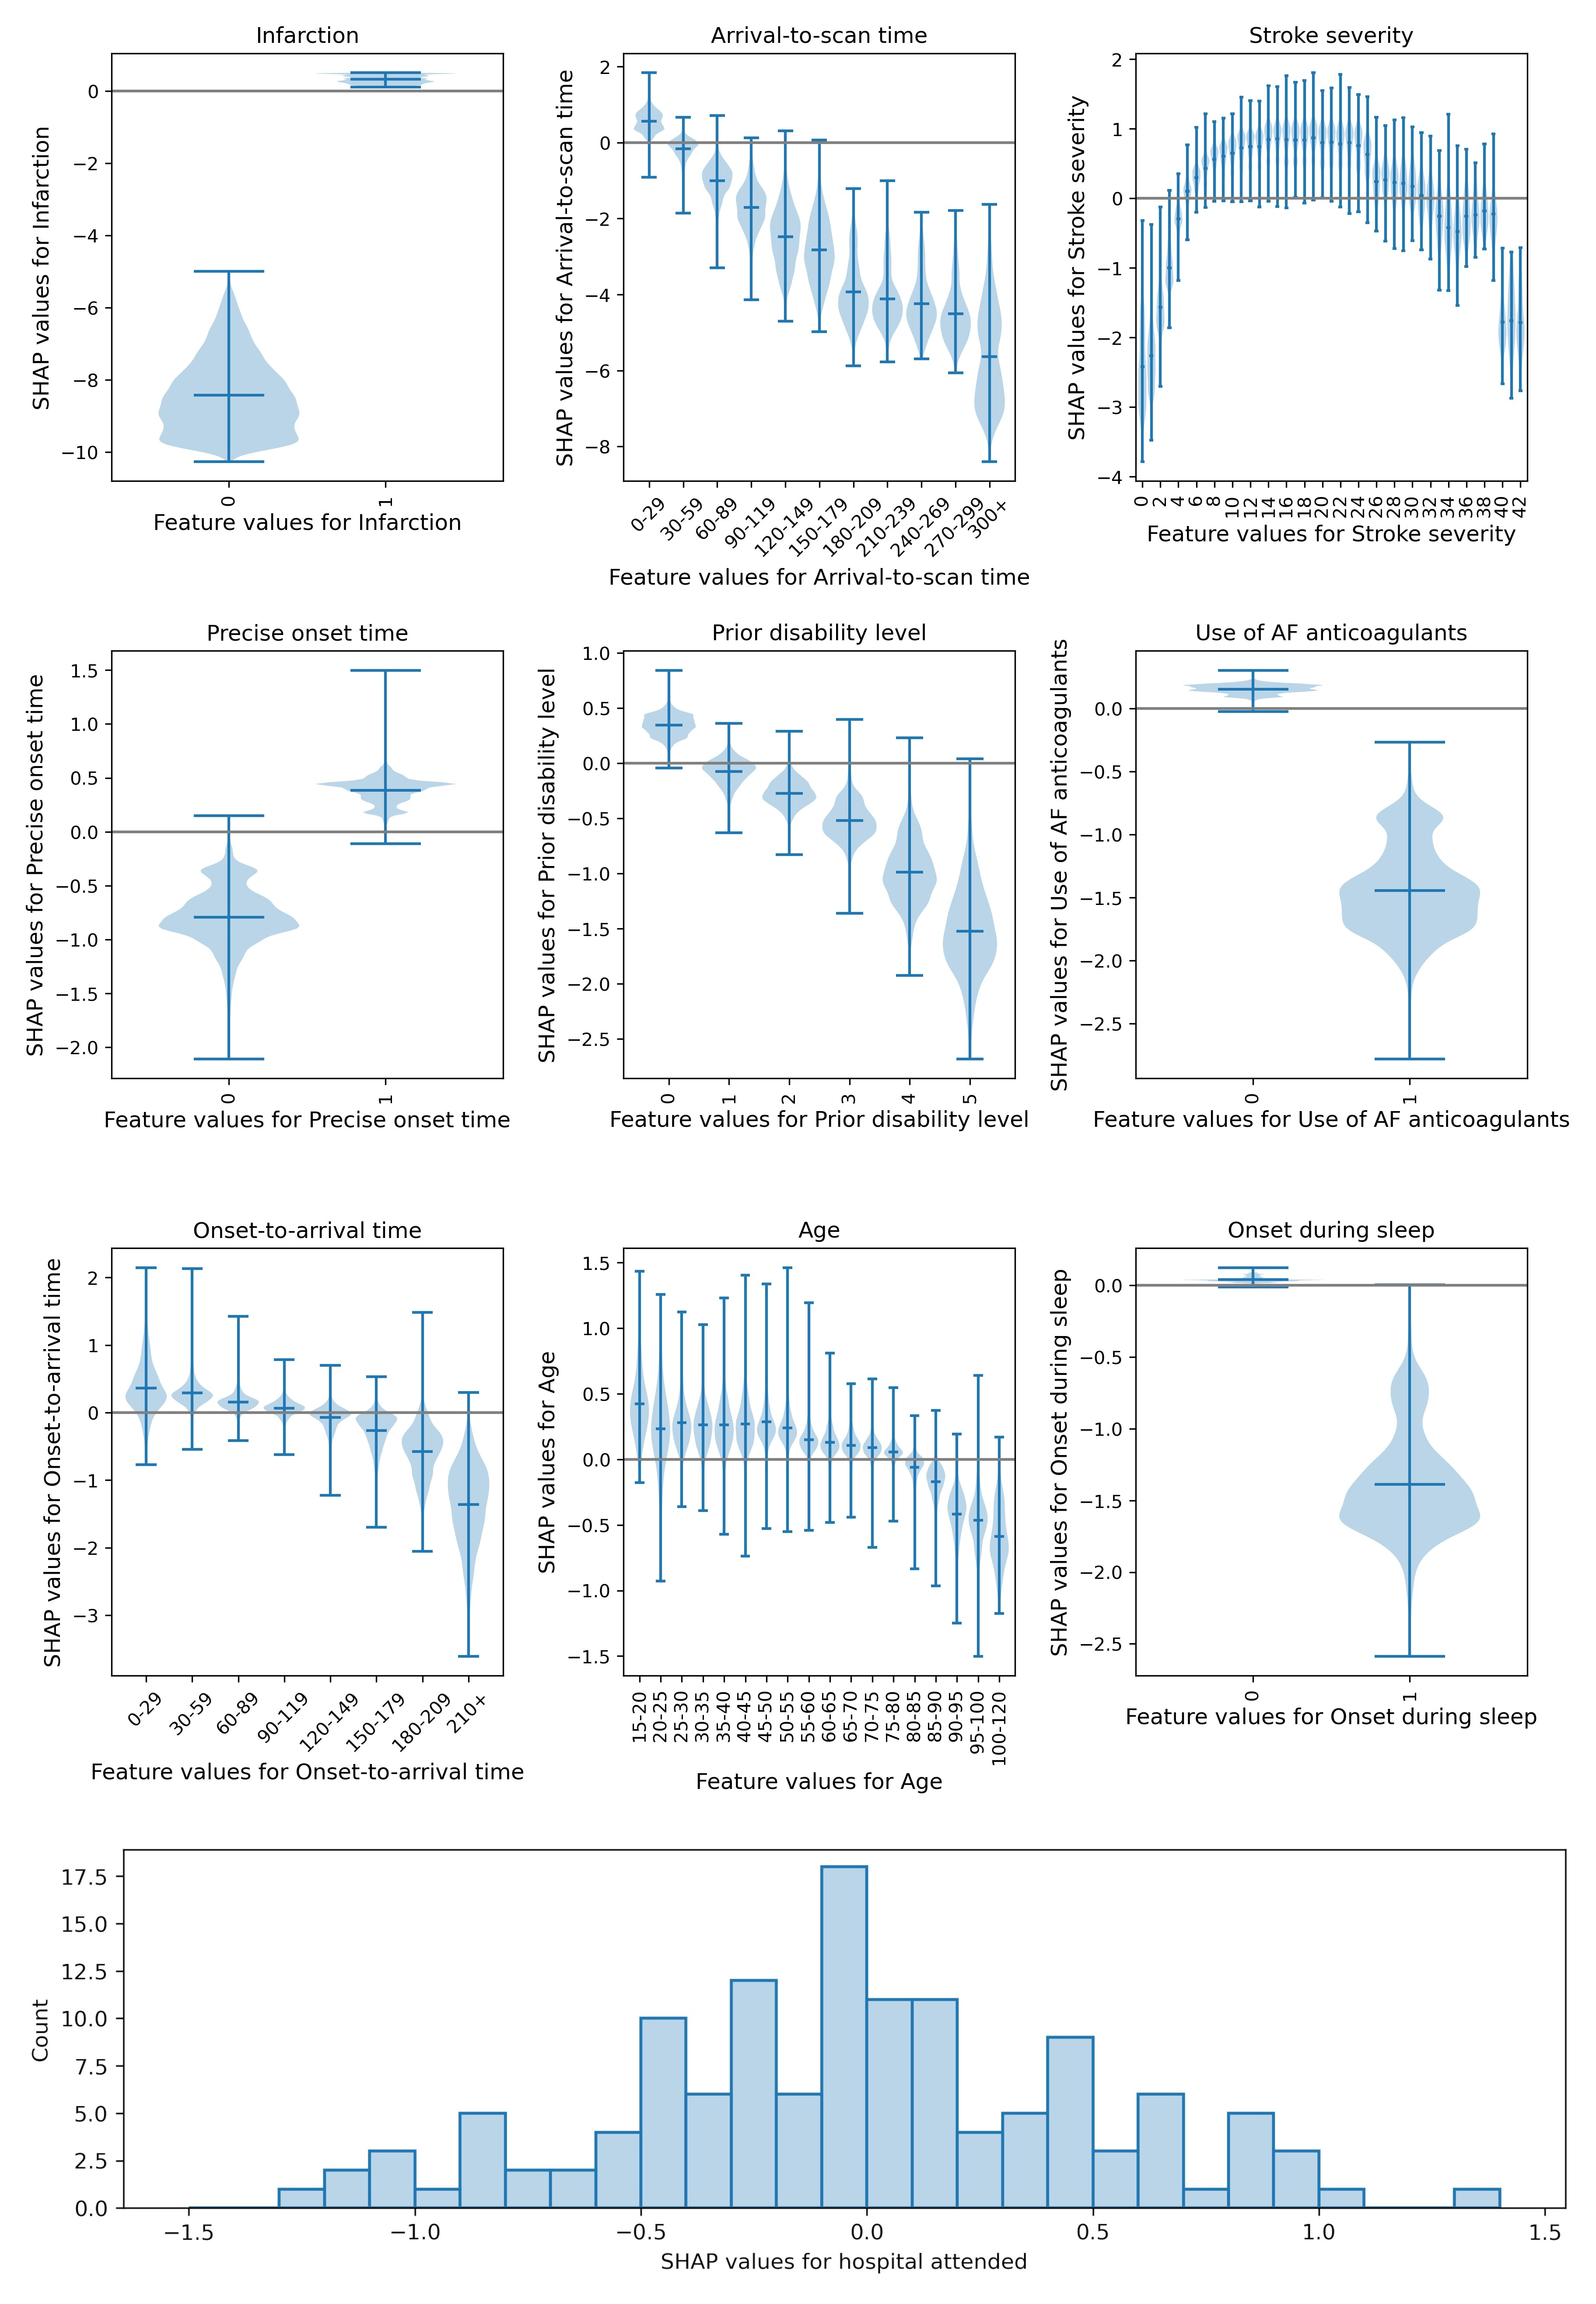
\includegraphics[width=0.85\textwidth]{./images/fig_1}
\caption{Plots showing the relationship between feature values and how the log-odds of receiving thrombolysis are effected (the \textit{SHAP} value). A SHAP value above zero represents an increased likelihood to receive thrombolysis, and a SHAP value below zero represents a decreased likelihood to receive thrombolysis. Top: Violin plots showing the relationship between SHAP values and feature values. The horizontal blue line shows the median SHAP value. The black horizontal line marks the SHAP value of zero. The plots are ordered in ranked feature importance (using the mean absolute SHAP value across all instances). Bottom: Histogram showing the frequency of SHAP values for the hospital attended.}
\label{fig:shap}
\end{figure}

We are developing a web app (available at \url{https://stroke-predictions.streamlit.app/}) that allows teams to compare their thrombolysis use decisions with the decisions made at other hospitals, across the full spectrum of patient characteristics. The web app also allows teams to see how changing pathway process speeds, or changing the ascertainment of the stroke onset time, or changing decision-making, may change thrombolysis use and outcomes at their hospital.

% 3) What do we not know

Current NIHR-funded work (\url{https://fundingawards.nihr.ac.uk/award/NIHR134326}) is focussing on building explainable machine learning models to predict death and disability-level outcomes with and without thrombolysis (and with differing time to thrombolysis). The observational data set we are using has over 40,000 patients receiving thrombolysis, compared to 6,756 in the seminal meta-analysis conducted by Emberson \textit{et al.} \cite{emberson_effect_2014}. Use of observational data also allows the investigation of the effect of thrombolysis as use is extended outside of clinical trial inclusion criteria. 

Some patterns are appearing in the analysis which may help guide clinicians on use of thrombolysis. In mild stroke (which was not generally included in the clinical trials), we observe that early thrombolysis is associated with a reduced chance of death, whereas later thrombolysis is associated with an increased chance of death (fig \ref{fig:death}). It is possible, however, that this effect is co-incidental rather than causal. We therefore wish to strengthen this type of analysis, by combining explainable machine learning with a range of causal inference methods.

\begin{figure}
\centering
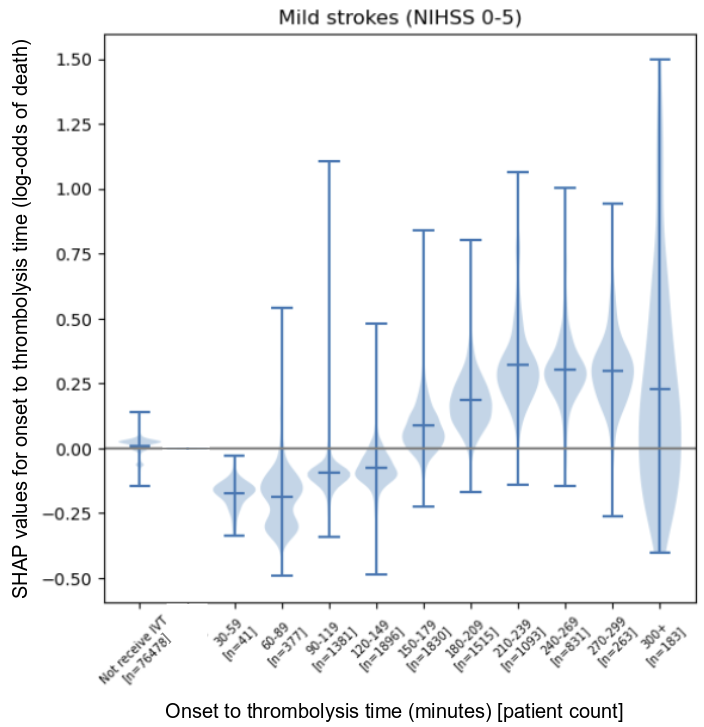
\includegraphics[width=0.5\textwidth]{./images/fig_2_}
\caption{Violin plot showing the relationship between time to thrombolysis and and how the log-odds of death are effected (the \textit{SHAP} value) in mild strokes. A mild stroke is defined as a National Institutes of Health Stroke Scale (NIHSS) 0-5.}
\label{fig:death}
\end{figure}

\section{Research aims}

The key aim of the proposed research is to incorporate causal inference methodology into our clinical pathway simulation and explainable machine learning analysis of emergency stroke care. We consider this a key methodological development, alongside explainable machine learning, to test, and build trust in, how changes in use of thrombolysis will effect patient outcomes.

\subsection{Specific research questions}

We are interested in incorporating causal inference analysis into a wide range of our work, but we have specific research questions to pin this development to. These research questions will help ensure advice given to stroke teams has the strongest foundations for improving outcomes.

\begin{itemize}
    \item In subgroups of patients where we see significant inter-hospital variation in use of thrombolysis, is there good evidence that the hospital is causing the variation in thrombolysis use in these groups (rather than this effect coinciding with other factors)? Example patient subgroups are 1) mild stroke (at presentation), 2) presence of prior disability, and 3) imprecisely known stroke onset time.

    \item In subgroups of patients where we see significant changes in outcome, is there good evidence that the main feature of interest in the patient subgroup is causing the variation in outcome in these groups (rather than this effect coinciding with other factors)? Example patient subgroups include early vs. late thrombolysis in mild stroke (where early thrombolysis appears to reduce the odds of death, but late thrombolysis increases the odds of death)?
\end{itemize}


\section{Project plan}

\subsection{Data}

We use anonymous patient-level data from the Sentinel Stroke National Audit Programme (SSNAP, \url{https://www.strokeaudit.org/}). SSNAP collects data from all emergency stroke units in England, Wales, and Northern Ireland. The data includes a wide range of information such as data on times throughout the stroke pathway from stroke onset, pre-stroke disability (modified Rankin Scale, mRS), a breakdown of stroke symptoms using the NIHSS stroke scale, reperfusion treatment given (and timing), comorbidities, death in hospital, disability at discharge from inpatient care, and 6 month follow-up disability (the latter is complete for about 35\% of discharged patients). Data is collected for about 85,000 patients each year, 10-11\% of whom receive thrombolysis.

\subsection{Methods}

When using observational data, no single method can provide proof of causality. Instead we will use a series of methods, each of which will contribute to understand causality. These methods will be applied to choice of thrombolysis, and outcomes, especially where we have identified high between-hospital variation in the use of thrombolysis. 

\begin{itemize}

    \item \textbf{Explainable machine learning with SHAP} \cite{aas_explaining_2020} - We will continue to use SHAP analyse to provide machine learning models at a global level and for individual predictions.

    \item \textbf{DAG (directed acyclic graphs)} \cite{tennant_use_2021} - Articulating proposed causal relationships through use of DAGs help to make assumed or hypothesised causal and non-causal relationships clear. They are easily understood by non-technical audiences, and so form an excellent basis for discussions and workshops to explore proposed causal relationships with clinical experts. We will use these, alongside results from other methods, in co-production workshops.
    
    \item \textbf{Target trial emulation} \cite{bigirumurame_current_2023} - This method involves mimicking the original thrombolysis clinical trials from observational data, using the original trial inclusion criteria, and then extending to groups that were not included in the original trial.

    \item \textbf{Natural experiments} \cite{craig_natural_2017} - Natural experiments compare outcomes when changes in services in any hospital are known to have occurred. We may, for example, look for shifts in thrombolysis use in individual hospitals and investigate outcomes.

    \item \textbf{Covariate adjustment} \cite{igelstrom_causal_2022} - We will identify all of the potential confounding variables, and include all of them that we can in a predictive model. Confounders are features, such as stroke severity, that affect both the probability of receiving thrombolysis, and the patient outcome. 

    \item \textbf{Use of propensity score as an adjusting feature} \cite{rosenbaum_central_1983} - \textit{`Propensity'}, the likelihood of a person receiving thrombolysis (estimated from a separate machine learning model), is added to the outcome prediction model, allowing the outcome model to be adjusted for patients' suitability for treatment. This helps to identify, and correct for, better outcomes occurring in patients suitable for thrombolysis, even if they did not receive thrombolysis.

    \item \textbf{Matching} - Creation of matched populations of control and test patients. Matching attempts to create cohorts of patients that are similar in both groups apart from the feature with proposed causal influence, allowing for an estimation of the effect of the causal feature under study. Matching may be performed using nearest-neighbour approaches \cite{stuart_matching_2010} or by propensity scores \cite{rosenbaum_central_1983}.

    \item \textbf{Stratification of results by propensity score} \cite{rosenbaum_central_1983} - Allowing comparisons of groups of patients who have similar suitability for treatment with thrombolysis.

    \item \textbf{Instrumental variable analysis} \cite{stel_instrumental_2013} - This method compares outcomes depending on an 'instrument' that does not directly effect outcome, but effects the proposed causal feature. In our current model we isolate how a hospital affects the likelihood that a patient will be given thrombolysis; we will test this as an instrument to investigate whether there is a relationship between this feature and outcomes. This could provide a novel link between advanced explainable machine learning methods and causal inference work.
           
    \item \textbf{Inverse propensity weighting} \cite{glynn_introduction_2010} - Weighting the contribution of patients to the final outcome measurement based on their likelihood of receiving, or not-receiving, thrombolysis. This method gives most weight to patients who received thrombolysis, who are more like patients who usually do not receive thrombolysis (and \textit{vice versa}). It also gives more weight to patients who are borderline in whether they would receive treatment or not.   
       
    \item \textbf{Double machine learning} \cite{chernozhukov_doubledebiased_2017} - This method combines two machine learning models, one to predict use of treatment and the other to predict outcome from that treatment. The treatment model estimates the probability of treatment given the observed covariates, while the outcome model estimates the expected outcome given the observed covariates and treatment. The errors (residuals) in the models are used as surrogates for missing information in each model. This method isolates a features causal relationship with the outcome by fitting the residuals of the feature prediction to the residuals of the outcomes.
\end{itemize}

All work will be performed in Python using established libraries for each of the methods (especially the \textit{XGBoost}, \textit{SHAP}, \textit{DoWhy} and \textit{EconML} libraries). Work will be conducted in \textit{Jupyter notebooks}, all of which will be published in an online \textit{Jupyter Book}.

\subsection{Co-production with the NHS, and link to patient benefit}

During this project we will hold stakeholder workshops to obtain feedback on the work. This will use our existing stakeholder network across the SSNAP, Integrated Stroke Delivery Networks (ISDN) and Integrated Care Systems (ICS). As we are working alongside NHS-England and NHS-Elect with teams with low thrombolysis (see paragraph below), we will also use this experience to refine project outputs.

A pilot web portal is being made available from autumn 2023, providing analysis of thrombolyis use at each hospital, comparing their hospital decisions to the decisions made at other hospitals. Modelling will also show how changing any combination of 1) process speeds, 2) ascertainment of stroke onset time, or 3) clinical decision making, would likely effect thrombolysis use and outcomes (based on a mathematical model of outcome depending on time to thrombolysis).

The modelling work currently being performed (\url{https://fundingawards.nihr.ac.uk/award/NIHR134326}) is planned to be incorporated into the national stroke audit from spring 2024. This will provide teams with a 
 realistic target thrombolysis use for their own patient population, and identify which area of the stroke pathway to focus on (for example pathway speed, ascertainment of stroke onset time, thrombolysis decision making). Additionally, NHS-Elect (who are working with NHS-England, the SAMueL team, and the national stroke audit) have an NHS improvement target to “Improve access to thrombolysis such that by the end of 2027/28, 20\% of stroke patients will receive thrombolysis treatment”. This collaborative will be working with 6 low-thrombolysing teams in the first instance, before extending work to all emergency stroke teams. As part of the quality improvement work, the SAMueL team will be providing modelling on use of thrombolysis, including on variation in decision-making between hospitals. We consider it important that this work should, if at all possible, include strengthened work on causality (the links between changes to pathway and decision making, through to thrombolysis use, and through to outcome) so that we have greater confidence that changes suggested (and potentially made) will lead to the expected improvement in thrombolysis use and, most importantly, in better outcomes and not 'just' increased thrombolysis use.

\subsection{Dissemination}

In addition to working with the national stroke audit and stroke teams directly (see above), we will also publish our work in leading stroke journals, and present it at stroke conferences. All of our detailed work is published online (e.g. see \url{https://samuel-book.github.io/samuel_shap_paper_1}).

\subsection{Project team}

The project team brings together experience of stroke care, machine learning, epidemiology, public and patient involvement, clinical trials, and causal inference work.

\begin{itemize}

    \item \textbf{Michael Allen (Co-PI, 25\% FTE)} co-leads our NIHR funded work on explainable machine learning (\url{https://fundingawards.nihr.ac.uk/award/NIHR134326}), with a focus on the technical aspects of the project. MA has extensive experience of health systems modelling and machine learning.

    \item \textbf{Kerry Pearn (Co-PI, 50\% FTE)} has been the principal developer of our explainable machine learning methodology for prediction of thrombolysis use and outcome. KP will co-lead the proposed work, with a focus on detailed work planning and execution, bringing in advice from co-investigators.

    \item \textbf{Martin James (Co-I, 5\% FTE)} is a stroke consultant and clinical director of the national stroke audit. Prof James co-leads our NIHR funded work on explainable machine learning (\url{https://fundingawards.nihr.ac.uk/award/NIHR134326}), with a focus on clinical oversight of the project. MJ will provide clinical oversight for this proposed project.

    \item \textbf{Mark Kelson (Co-I, 5\% FTE)} is a statistician working in the overlap between clinical trials, medical statistics, causal inference, reproducibility and data science. MK will advise on statistics and causal inference methods.

    \item \textbf{João Delgado (Co-I, 10\% FTE)} is an epidemiologist focusing on management of conditions affecting cognitive function in old age, using traditional and modern epidemiology and statistical tools to analyse large datasets of electronic health records. JD will advise on epidemiological methodologies such as use of propensity scores.

    \item \textbf{Lauren Asare (Researcher, 5\%)} is a research assistant in the University of Exeter PenARC Public and Patient involvement team. LA supports our stroke patient and carer involvement (PCI) team (which is chaired by a stroke survivor).

\end{itemize}

\subsection{Patient and carer involvement}

Our team has a dedicated PCI group who provide constant input into our work and have provided input to this bid. The PCI group have been a key voice in guiding our work to look at what maximises patient outcomes, and not arbitrary targets on thrombolysis use. The PCI team is chaired by Leon Farmer, a stroke supervisor, with guidance from Lauren Asare of the University of Exeter PenARC PPI team.

\subsection{People development}

In addition to development of the methodology, this project will be used to develop the skills and capabilities of Kerry Pearn (Co-PI) who will lead the project with assistance from Michael Allen (Co-PI). The stroke modelling and data science team is a stable team, funded by research grants and NHS-contracted work, and the techniques and skills developed here will find long-term use and benefit.

\subsection{Contribution beyond this project}

We work on a range of projects that would benefit from this method development in our work. For example, we are working on stroke projects focusing on the pre-hospital pathway (\url{https://fundingawards.nihr.ac.uk/award/NIHR202361}) and the use of mobile stroke units (\url{https://fundingawards.nihr.ac.uk/award/NIHR153982}). The methodological development above will add value to both of these, and also to other similar, projects. For example, it has previously been assumed that outcome from haemorrhagic stroke (the 20\% of strokes that are caused by a bleed rather than a clot) is independent of ambulance travel time, but some recent clinical trials on taking stroke patients further, to a hospital with more capabilities for strokes caused by clots, have suggested this may not be true. Using methods such as clinical trial emulation and our large database of stroke data we will have the potential to enhance our pre-hospital stroke care model to better model outcomes of haemorrhagic strokes with alternative pre-hospital pathways.

\section{Intellectual property}

We work on a principal that public funding should give public benefit, and so all our detailed work (code) is shared with an Open Licence, allowing anyone to use or develop it.
